\documentclass[11pt,]{article}
\usepackage[left=1in,top=1in,right=1in,bottom=1in]{geometry}
\newcommand*{\authorfont}{\fontfamily{phv}\selectfont}



\usepackage[]{mathpazo}


  \usepackage[T1]{fontenc}
  \usepackage[utf8]{inputenc}

\usepackage{abstract}
\renewcommand{\abstractname}{}    % clear the title
\renewcommand{\absnamepos}{empty} % originally center

\renewenvironment{abstract}
 {{%
    \setlength{\leftmargin}{0mm}
    \setlength{\rightmargin}{\leftmargin}%
  }%
  \relax}
 {\endlist}

\makeatletter
\def\@maketitle{%
  \newpage
%  \null
%  \vskip 2em%
%  \begin{center}%
  \let \footnote \thanks
    {\fontsize{18}{20}\selectfont\raggedright  \setlength{\parindent}{0pt} \@title \par}%
}
%\fi
\makeatother




\setcounter{secnumdepth}{0}



\title{Lab 5: Biodiversity \thanks{\textbf{Current version}: April , 2019}  }



\author{\Large BIO 3103, Baylor University\vspace{0.05in} \newline\normalsize\emph{}  }


\date{}

\usepackage{titlesec}

\titleformat*{\section}{\Large\bfseries}
\titleformat*{\subsection}{\normalsize\itshape}
\titleformat*{\subsubsection}{\normalsize\itshape}
\titleformat*{\paragraph}{\normalsize\itshape}
\titleformat*{\subparagraph}{\normalsize\itshape}





\newtheorem{hypothesis}{Hypothesis}
\usepackage{setspace}

\makeatletter
\@ifpackageloaded{hyperref}{}{%
\ifxetex
  \PassOptionsToPackage{hyphens}{url}\usepackage[setpagesize=false, % page size defined by xetex
              unicode=false, % unicode breaks when used with xetex
              xetex]{hyperref}
\else
  \PassOptionsToPackage{hyphens}{url}\usepackage[unicode=true]{hyperref}
\fi
}

\@ifpackageloaded{color}{
    \PassOptionsToPackage{usenames,dvipsnames}{color}
}{%
    \usepackage[usenames,dvipsnames]{color}
}
\makeatother
\hypersetup{breaklinks=true,
            bookmarks=true,
            pdfauthor={BIO 3103, Baylor University ()},
             pdfkeywords = {},  
            pdftitle={Lab 5: Biodiversity},
            colorlinks=true,
            citecolor=blue,
            urlcolor=blue,
            linkcolor=magenta,
            pdfborder={0 0 0}}
\urlstyle{same}  % don't use monospace font for urls

% set default figure placement to htbp
\makeatletter
\def\fps@figure{htbp}
\setlength{\intextsep}{25pt}  % sets space after text/before float figure
\makeatother

\usepackage{multicol}
\usepackage{textcomp}
\usepackage{textgreek}
\usepackage{pdflscape}
\usepackage{float}
\usepackage{booktabs}
\usepackage{makecell}
\usepackage[table]{xcolor}
\usepackage{fixltx2e}
\usepackage{hyperref}
\usepackage{graphicx}


% add tightlist ----------
\providecommand{\tightlist}{%
\setlength{\itemsep}{0pt}\setlength{\parskip}{0pt}}

\begin{document}
	
% \pagenumbering{arabic}% resets `page` counter to 1 
%


% \maketitle

{% \usefont{T1}{pnc}{m}{n}
\setlength{\parindent}{0pt}
\thispagestyle{plain}
{\fontsize{18}{20}\selectfont\raggedright 
\maketitle  % title \par  

}

{
   \vskip 13.5pt\relax \normalsize\fontsize{11}{12} 
\textbf{\authorfont BIO 3103, Baylor University} \hskip 15pt \emph{\small }   

}

}




\noindent  \section{Background information}\label{background-information}

Quantifying biodiversity is an active area of research for ecologists
and conservationists. Organisms have evolved alongside each other, and
developed adaptations that allow them to thrive in different niches. The
interactions between these organisms, and between these organisms and
their environment can be incredibly complex. How diverse communities
are, and how diversity changes area to area, can tell us a lot about an
ecosystem. How do we even measure diversity? Or how similar 2 areas are?
Alpha-diversity is a measure of biodiversity at a single location, while
gamma-diversity is the cumulative diversity in a particular region of
interest. Beta-diversity links the two, and is a measure of variable
community composition is among locations (Fig. 1).

\begin{figure}

{\centering 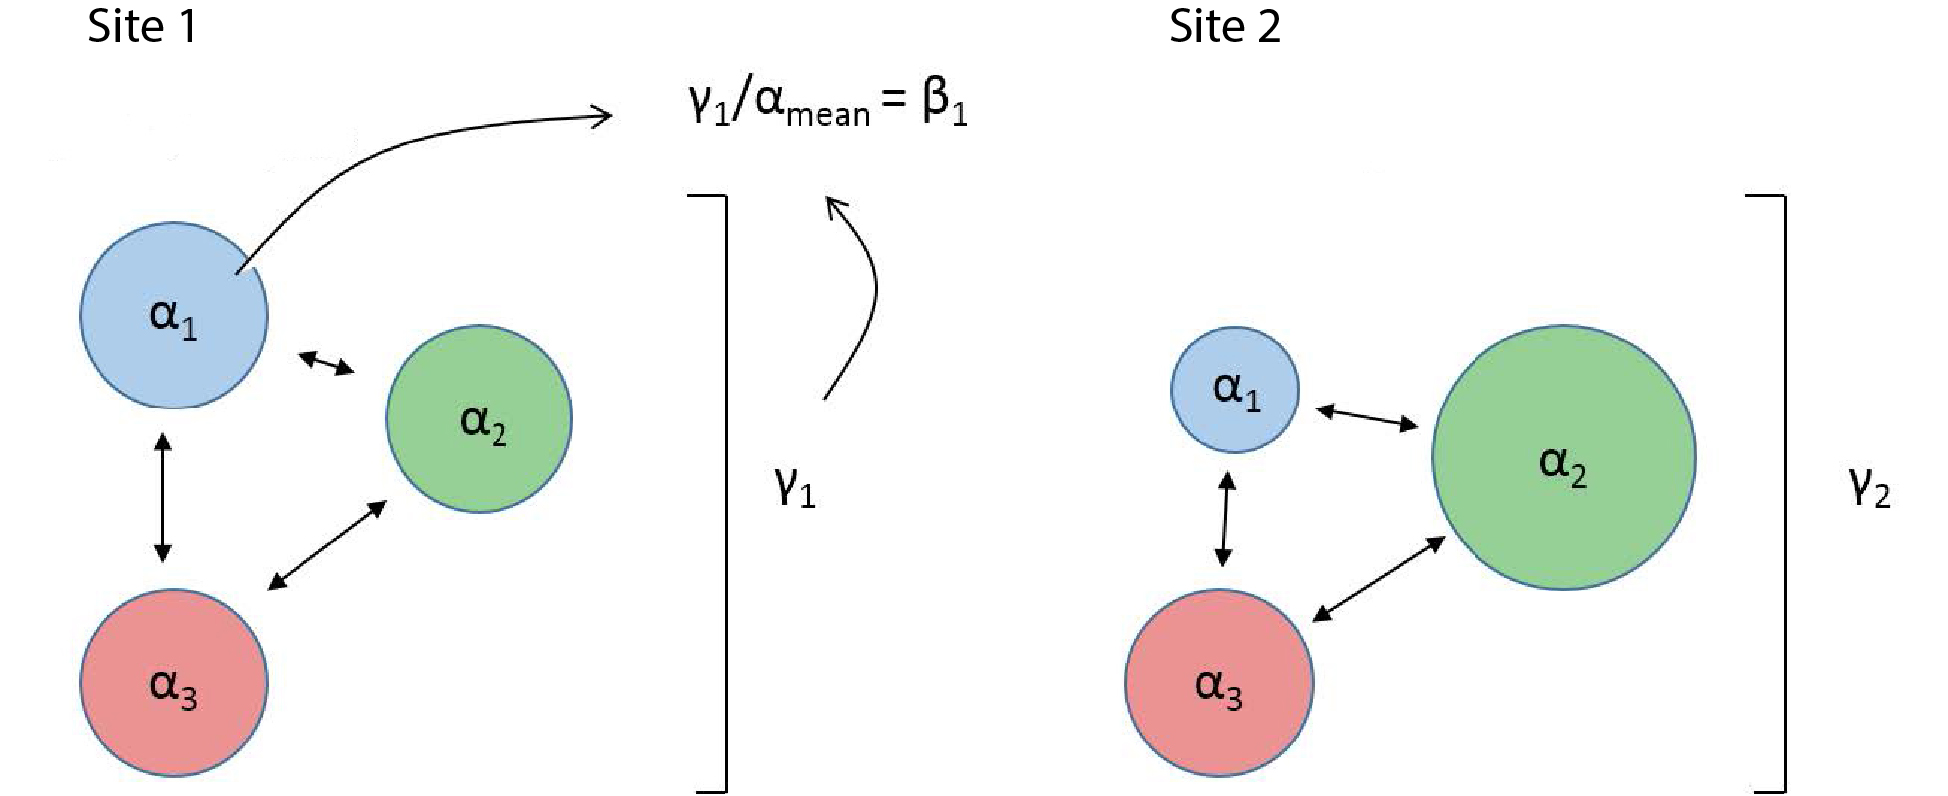
\includegraphics[width=1\linewidth]{../_chapter_materials/partitioning} 

}

\caption{Schematic representation of how alpha (sample level), gamma (region level), and beta (sample variability) diversities are related. For each stream you have multiple measures of alpha-diversity (taxa richness), with one measure of gamma and beta-diversity per stream.}\label{fig:partition-fig}
\end{figure}

There are many ways to quantify biodiversity, and scientists have been
discussing (i.e.~arguing) about the best way to go about it for years,
but at its heart all biodiversity metrics are a way to compress complex
information into an interpretable number. A coarse analogy would be the
Body Mass Index (BMI) score. Humans are comprised of assemblages of
cells and organ systems, and we could measure the health of a single
individual in thousands of different ways. The BMI score is a simple way
to compress that information into a single number that we can use to
assess relative `health'. We can do something similar for biodiversity!
I do not want you to conflate `health' with `biodiversity', but it is a
useful starting point. For this lab we will use species richness (the
number of species) as our measure of biodiversity.

Benthic macroinvertebrates (Fig. 2) are a useful group of study
organisms because they are incredibly diverse, and are important
ecological indicators of the physical and chemical characteristics of
streams. Some are sensitive to changes in dissolved oxygen or pH, or
will struggle if sediment loads into the stream from the surrounding
landscape are too high. Stream ecosystems are linked to the areas around
them (their watershed). Think of some ways that humans influence the
landscape - then Google how those changes influence aquatic environments
(most anthropogenic impacts are very well studied).

\begin{figure}

{\centering 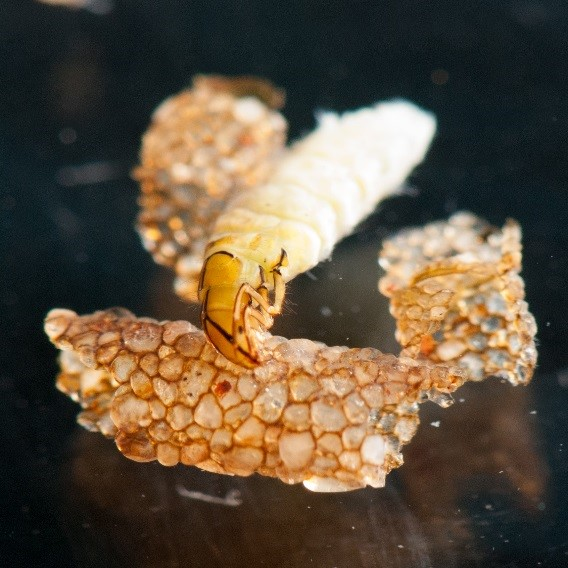
\includegraphics[width=0.5\linewidth]{../_chapter_materials/invert_pic} 

}

\caption{Example macroinvertebrate (Order: Trichoptera) that you will collect in the field and identify under a dissecting microscope. Caddisflies frequently have elaborate shells built from materials around them in the stream.}\label{fig:invert-fig}
\end{figure}

\section{Objectives}\label{objectives}

We collected macroinvertebrates from 2 sites in central Texas that
differed in anthropogenic impact using 1 m\textsuperscript{2}
kick-screens. The Middle Bosque, while it does have some farm and
pastureland in its watershed, it relatively undisturbed compared some
other streams in the area. Hog Creek is in an adjacent watershed, and
has slightly higher nutrient concentrations that cause large blooms of
nuisance filamentous algae. You will use this data to compare
biodiversity between the two sites and answer the following questions:

\begin{enumerate}
\def\labelenumi{\arabic{enumi}.}
\tightlist
\item
  Does anthropogenic impact influence mean alpha diversity?

  \begin{itemize}
  \tightlist
  \item
    Assess this question by calculating alpha-diversity. Display this
    information in a column graph, and use a t-test to determine if
    there are statistically signifiant differences between
    alpha-diversity of the two streams.
  \end{itemize}
\item
  Does anthropogenic impact influence gamma diversity?

  \begin{itemize}
  \tightlist
  \item
    Calculate gamma diversity for each stream and report these values in
    the text.
  \end{itemize}
\item
  Does anthropogenic impact influence beta diversity?

  \begin{itemize}
  \tightlist
  \item
    Calculate beta diversity for each stream and report these values in
    the text.
  \end{itemize}
\end{enumerate}

\section{Lab report specifics}\label{lab-report-specifics}

\begin{enumerate}
\def\labelenumi{\arabic{enumi}.}
\tightlist
\item
  Introduction

  \begin{itemize}
  \tightlist
  \item
    Why is biodiversity important?
  \item
    How is biodiversity measured?
  \item
    Why are macroinvertebrates useful?
  \item
    Objectives
  \item
    Hypotheses
  \end{itemize}
\item
  Methods

  \begin{itemize}
  \tightlist
  \item
    Experimental design and field work
  \item
    Laboratory work (macroinvertebrate processing and identification)
  \item
    Calculations / statistics
  \end{itemize}
\item
  Results

  \begin{itemize}
  \tightlist
  \item
    Question 1 (text \textbf{AND} graph)
  \item
    Question 2 (text)
  \item
    Question 3 (text)
  \end{itemize}
\item
  Discussion

  \begin{itemize}
  \tightlist
  \item
    Hypotheses rejected/supported
  \item
    Provide a coherent explanation/interpretation of your results
  \end{itemize}
\end{enumerate}




\newpage
\singlespacing 
\end{document}
